% MURU-BENCH: A Benchmark for Mathematical Reasoning Under Uncertainty
% NeurIPS 2026 Datasets and Benchmarks Track

\documentclass{article}

% NeurIPS style (download neurips_2026.sty from neurips.cc when available)
% For now, use a compatible setup
\usepackage[final]{neurips_2024}  % Replace with neurips_2026 when available

\usepackage[utf8]{inputenc}
\usepackage[T1]{fontenc}
\usepackage{hyperref}
\usepackage{url}
\usepackage{booktabs}
\usepackage{amsfonts}
\usepackage{amsmath}
\usepackage{nicefrac}
\usepackage{microtype}
\usepackage{graphicx}
\usepackage{xcolor}
\usepackage{subcaption}
\usepackage{algorithm}
\usepackage{algorithmic}

\title{MURU-BENCH: A Benchmark for Mathematical Reasoning Under Uncertainty}

% Authors — update before submission
\author{
  Author Name \\
  Affiliation \\
  \texttt{email@example.com}
}

\begin{document}

\maketitle

% ─────────────────────────────────────────────────────────────────
% ABSTRACT — Write this LAST
% ─────────────────────────────────────────────────────────────────
\begin{abstract}
Large language models are evaluated on numerous mathematical reasoning benchmarks, yet none rigorously test reasoning under \emph{genuine mathematical uncertainty}---problems requiring Bayesian inference, calibrated confidence intervals, and explicit uncertainty quantification. We introduce MURU-BENCH (\textbf{M}athematical \textbf{R}easoning \textbf{U}nder \textbf{U}ncertainty \textbf{Bench}mark), a curated dataset of 3{,}000 problems spanning five categories: Bayesian Updating, Conditional Probability Chains, Distribution Estimation, Decision Under Uncertainty, and Adversarial Ambiguity. Each problem requires a model to identify the correct probabilistic framework, execute multi-step mathematical reasoning, and produce a calibrated answer with a justified confidence interval. We evaluate [N] frontier and open-source models and find that [KEY FINDING 1] and [KEY FINDING 2]. MURU-BENCH fills a critical gap in the evaluation landscape and provides a rigorous measuring stick for progress in calibrated reasoning.

% TODO: Fill in specific findings after Phase 2 evaluation
\end{abstract}

% ─────────────────────────────────────────────────────────────────
% 1. INTRODUCTION
% ─────────────────────────────────────────────────────────────────
\section{Introduction}
\label{sec:introduction}

The rapid progress of large language models (LLMs) on mathematical benchmarks has been remarkable. Models now achieve near-human performance on GSM8K~\citep{gsm8k}, competitive results on MATH~\citep{math}, and broad knowledge on MMLU~\citep{mmlu}. However, these benchmarks share a fundamental limitation: they test reasoning toward \emph{single, deterministic correct answers}.

Real-world mathematical reasoning frequently involves \emph{genuine uncertainty}---not the colloquial sense of ``being unsure,'' but the precise mathematical sense of reasoning with probability distributions, unknown parameters, and ambiguous problem structure. A physician interpreting a diagnostic test must combine base rates with test characteristics. An engineer assessing failure risk must propagate uncertainty through a chain of conditional probabilities. A decision-maker must choose actions under uncertain utility functions.

No existing benchmark rigorously tests this capability. We identify this as the \textbf{calibrated uncertainty gap}: the absence of a mathematical benchmark that requires models to reason formally about probability while handling ambiguous problem structure, and to produce calibrated confidence in their answers.

MURU-BENCH fills this gap. Our contributions are:

\begin{enumerate}
    \item A curated dataset of 3{,}000 problems across five categories, each requiring genuine mathematical reasoning under uncertainty (Section~\ref{sec:dataset}).
    \item A comprehensive evaluation framework with six metrics, including Expected Calibration Error (ECE) and overconfidence rate, that measure not just accuracy but calibration quality (Section~\ref{sec:evaluation}).
    \item Baseline evaluations of [N] frontier and open-source models, revealing [KEY FINDING] (Section~\ref{sec:results}).
    \item Analysis of where and why models fail at uncertainty reasoning, with implications for AI safety and deployment (Section~\ref{sec:analysis}).
\end{enumerate}


% ─────────────────────────────────────────────────────────────────
% 2. RELATED WORK
% ─────────────────────────────────────────────────────────────────
\section{Related Work}
\label{sec:related}

\paragraph{Mathematical Reasoning Benchmarks.}
GSM8K~\citep{gsm8k} tests grade-school arithmetic with deterministic answers. MATH~\citep{math} covers competition-level problems across algebra, geometry, and number theory, but all problems have single correct answers. BIG-Bench Hard~\citep{bigbench} includes diverse reasoning tasks but lacks formal probability combined with ambiguity.

\paragraph{Calibration in Language Models.}
\citet{kadavath2022} showed that language models exhibit some knowledge of what they know. \citet{guo2017} established methods for measuring calibration in neural networks via Expected Calibration Error (ECE). Recent work has explored prompting strategies to elicit calibrated uncertainty~\citep{tian2023}, but no benchmark provides ground-truth calibration targets.

\paragraph{Uncertainty Quantification.}
The machine learning community has extensively studied predictive uncertainty~\citep{gal2016, lakshminarayanan2017}, but primarily in the context of model ensembles and Bayesian neural networks, not in evaluating an LLM's ability to \emph{reason about} uncertainty as a mathematical concept.

MURU-BENCH is, to our knowledge, the first benchmark that combines formal mathematical reasoning with genuine uncertainty quantification, requiring both correct answers \emph{and} calibrated confidence.


% ─────────────────────────────────────────────────────────────────
% 3. DATASET CONSTRUCTION
% ─────────────────────────────────────────────────────────────────
\section{Dataset Construction}
\label{sec:dataset}

\subsection{Problem Design Principles}

Each MURU-BENCH problem satisfies five criteria:
\begin{enumerate}
    \item \textbf{Unambiguous correctness}: A professional mathematician would agree the answer is correct given stated assumptions.
    \item \textbf{Measurable failure}: An overconfident model would fail in a quantifiable way.
    \item \textbf{Mathematical uncertainty}: The uncertainty is mathematical, not merely linguistic vagueness.
    \item \textbf{Active reasoning}: The problem cannot be solved by retrieval alone.
    \item \textbf{Non-trivial intervals}: The ground-truth confidence interval is non-degenerate.
\end{enumerate}

\subsection{Problem Categories}

\begin{table}[h]
\centering
\caption{MURU-BENCH problem categories and counts.}
\label{tab:categories}
\begin{tabular}{lrp{6cm}}
\toprule
\textbf{Category} & \textbf{Count} & \textbf{Description} \\
\midrule
Bayesian Updating & 700 & Prior beliefs revised by evidence with ambiguous likelihoods \\
Conditional Probability Chains & 600 & Multi-step conditioning with uncertain intermediates \\
Distribution Estimation & 600 & Inferring distributions from incomplete samples \\
Decision Under Uncertainty & 550 & Expected value with uncertain utility functions \\
Adversarial Ambiguity & 550 & Problems designed to exploit overconfident reasoning \\
\midrule
\textbf{Total} & \textbf{3{,}000} & \\
\bottomrule
\end{tabular}
\end{table}

\subsection{Problem Format}

Each problem consists of six components: (1) a natural-language stem with embedded quantitative information, (2) an explicit uncertainty specification, (3) the correct mathematical framework tag, (4) a ground-truth answer with full solution, (5) a calibration target (confidence interval at a specified level), and (6) a difficulty rating from 1--5.

\subsection{Quality Control}

% TODO: Describe the quality control process after it is completed
Problems were authored by [AUTHOR] and validated through [PROCESS]. Each problem was checked against the five design principles using an automated validation script and manual review by [N] reviewers.


% ─────────────────────────────────────────────────────────────────
% 4. EVALUATION METHODOLOGY
% ─────────────────────────────────────────────────────────────────
\section{Evaluation Methodology}
\label{sec:evaluation}

We evaluate models on six metrics:

\begin{table}[h]
\centering
\caption{Evaluation metrics for MURU-BENCH.}
\label{tab:metrics}
\begin{tabular}{llp{5cm}}
\toprule
\textbf{Metric} & \textbf{Type} & \textbf{Description} \\
\midrule
Accuracy@exact & Correctness & Answer falls within ground-truth CI \\
ECE & Calibration & Expected Calibration Error (binned) \\
Category Breakdown & Diagnostic & Accuracy per problem category \\
Difficulty Scaling & Diagnostic & Accuracy by difficulty level \\
Overconfidence Rate & Safety & Fraction of high-confidence wrong answers \\
Framework Match & Process & Correct reasoning framework identified \\
\bottomrule
\end{tabular}
\end{table}

\paragraph{Prompting Protocol.}
% TODO: Describe the exact prompting protocol used for evaluation


% ─────────────────────────────────────────────────────────────────
% 5. RESULTS
% ─────────────────────────────────────────────────────────────────
\section{Results}
\label{sec:results}

% TODO: Fill in after Phase 2 evaluation is complete

\begin{table}[h]
\centering
\caption{Model performance on MURU-BENCH (test set, $n=300$).}
\label{tab:results}
\begin{tabular}{lccccc}
\toprule
\textbf{Model} & \textbf{Accuracy} & \textbf{ECE} $\downarrow$ & \textbf{Overconf.} $\downarrow$ & \textbf{Framework} & \textbf{Overall} \\
\midrule
GPT-4o & -- & -- & -- & -- & -- \\
Claude 3.5 Sonnet & -- & -- & -- & -- & -- \\
Gemini 1.5 Pro & -- & -- & -- & -- & -- \\
Llama 3 & -- & -- & -- & -- & -- \\
Mistral & -- & -- & -- & -- & -- \\
Qwen2-Math & -- & -- & -- & -- & -- \\
\bottomrule
\end{tabular}
\end{table}


% ─────────────────────────────────────────────────────────────────
% 6. ANALYSIS
% ─────────────────────────────────────────────────────────────────
\section{Analysis}
\label{sec:analysis}

% TODO: Fill in after Phase 2

\subsection{Where Do Models Fail?}

\subsection{Calibration Analysis}

\subsection{Difficulty Scaling}


% ─────────────────────────────────────────────────────────────────
% 7. LIMITATIONS
% ─────────────────────────────────────────────────────────────────
\section{Limitations}
\label{sec:limitations}

\begin{itemize}
    \item \textbf{Single author}: The majority of problems were authored by a single individual, which may introduce systematic biases in problem style and difficulty calibration.
    \item \textbf{English only}: All problems are in English, limiting the benchmark's applicability to multilingual evaluation.
    \item \textbf{Category scope}: While five categories cover the major types of mathematical uncertainty, domains such as stochastic processes and measure-theoretic probability are not represented.
    \item \textbf{Ground truth subjectivity}: For some Adversarial Ambiguity problems, the ``correct'' answer depends on modeling assumptions, which we address by providing answer ranges.
\end{itemize}


% ─────────────────────────────────────────────────────────────────
% 8. CONCLUSION
% ─────────────────────────────────────────────────────────────────
\section{Conclusion}
\label{sec:conclusion}

We introduced MURU-BENCH, the first benchmark for mathematical reasoning under genuine uncertainty. Our evaluation of [N] models reveals [KEY FINDING]. We release the full dataset, evaluation code, and baseline results to facilitate future research on calibrated reasoning in language models.


% ─────────────────────────────────────────────────────────────────
% REFERENCES
% ─────────────────────────────────────────────────────────────────
\bibliographystyle{plainnat}

\begin{thebibliography}{10}

\bibitem[Cobbe et al.(2021)]{gsm8k}
Karl Cobbe, Vineet Kosaraju, Mohammad Bavarian, Mark Chen, Heather Jun, Lukasz Kaiser, Matthias Plappert, Jerry Tworek, Jacob Hilton, Reiichiro Nakano, Christopher Hesse, and John Schulman.
\newblock Training verifiers to solve math word problems.
\newblock \emph{arXiv preprint arXiv:2110.14168}, 2021.

\bibitem[Hendrycks et al.(2021a)]{math}
Dan Hendrycks, Collin Burns, Saurav Kadavath, Akul Arora, Steven Basart, Eric Tang, Dawn Song, and Jacob Steinhardt.
\newblock Measuring mathematical problem solving with the MATH dataset.
\newblock In \emph{NeurIPS}, 2021.

\bibitem[Hendrycks et al.(2021b)]{mmlu}
Dan Hendrycks, Collin Burns, Steven Basart, Andy Zou, Mantas Mazeika, Dawn Song, and Jacob Steinhardt.
\newblock Measuring massive multitask language understanding.
\newblock In \emph{ICLR}, 2021.

\bibitem[Suzgun et al.(2023)]{bigbench}
Mirac Suzgun, Nathan Scales, Nathanael Sch{\"a}rli, Sebastian Gehrmann, Yi Tay, Hyung Won Chung, Aakanksha Chowdhery, Quoc Le, Ed Chi, Denny Zhou, and Jason Wei.
\newblock Challenging BIG-Bench tasks and whether chain-of-thought can solve them.
\newblock In \emph{ACL Findings}, 2023.

\bibitem[Kadavath et al.(2022)]{kadavath2022}
Saurav Kadavath, Tom Conerly, Amanda Askell, Tom Henighan, Dawn Drain, Ethan Perez, Nicholas Schiefer, Zac Hatfield-Dodds, Nova DasSarma, Eli Tyre, et al.
\newblock Language models (mostly) know what they know.
\newblock \emph{arXiv preprint arXiv:2207.05221}, 2022.

\bibitem[Guo et al.(2017)]{guo2017}
Chuan Guo, Geoff Pleiss, Yu Sun, and Kilian Q.\ Weinberger.
\newblock On calibration of modern neural networks.
\newblock In \emph{ICML}, 2017.

\bibitem[Tian et al.(2023)]{tian2023}
Katherine Tian, Eric Mitchell, Allan Dafoe, Anca Dragan, and Yejin Choi.
\newblock Just ask for calibration: Strategies for eliciting calibrated confidence scores from language models.
\newblock In \emph{EMNLP}, 2023.

\bibitem[Gal and Ghahramani(2016)]{gal2016}
Yarin Gal and Zoubin Ghahramani.
\newblock Dropout as a Bayesian approximation: Representing model uncertainty in deep learning.
\newblock In \emph{ICML}, 2016.

\bibitem[Lakshminarayanan et al.(2017)]{lakshminarayanan2017}
Balaji Lakshminarayanan, Alexander Pritzel, and Charles Blundell.
\newblock Simple and scalable predictive uncertainty estimation using deep ensembles.
\newblock In \emph{NeurIPS}, 2017.

\end{thebibliography}


% ─────────────────────────────────────────────────────────────────
% APPENDIX
% ─────────────────────────────────────────────────────────────────
\appendix

\section{Dataset Statistics}
\label{app:statistics}

% TODO: Insert generated figures from paper/figures/

\begin{figure}[h]
\centering
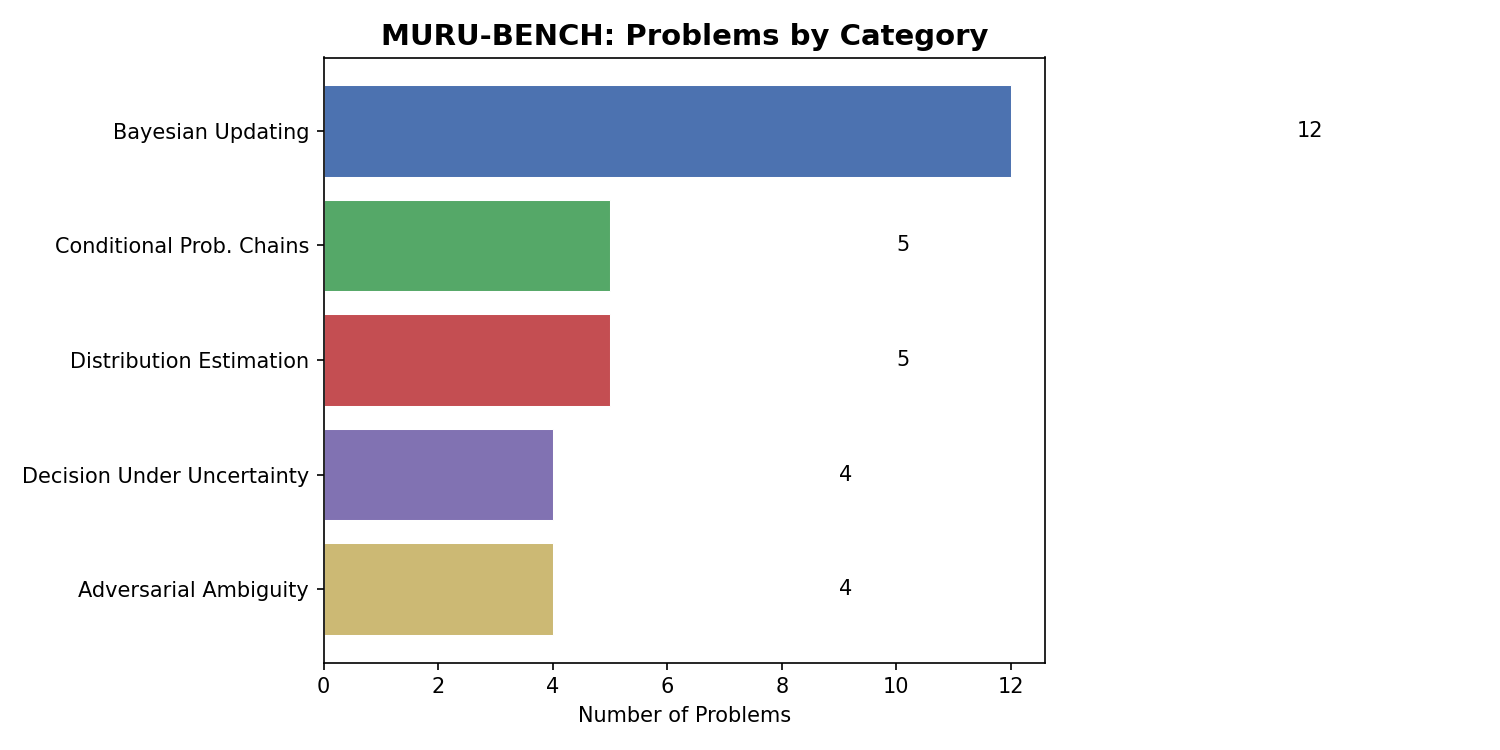
\includegraphics[width=0.7\textwidth]{figures/category_distribution.png}
\caption{Distribution of problems by category in MURU-BENCH.}
\label{fig:category_dist}
\end{figure}

\begin{figure}[h]
\centering
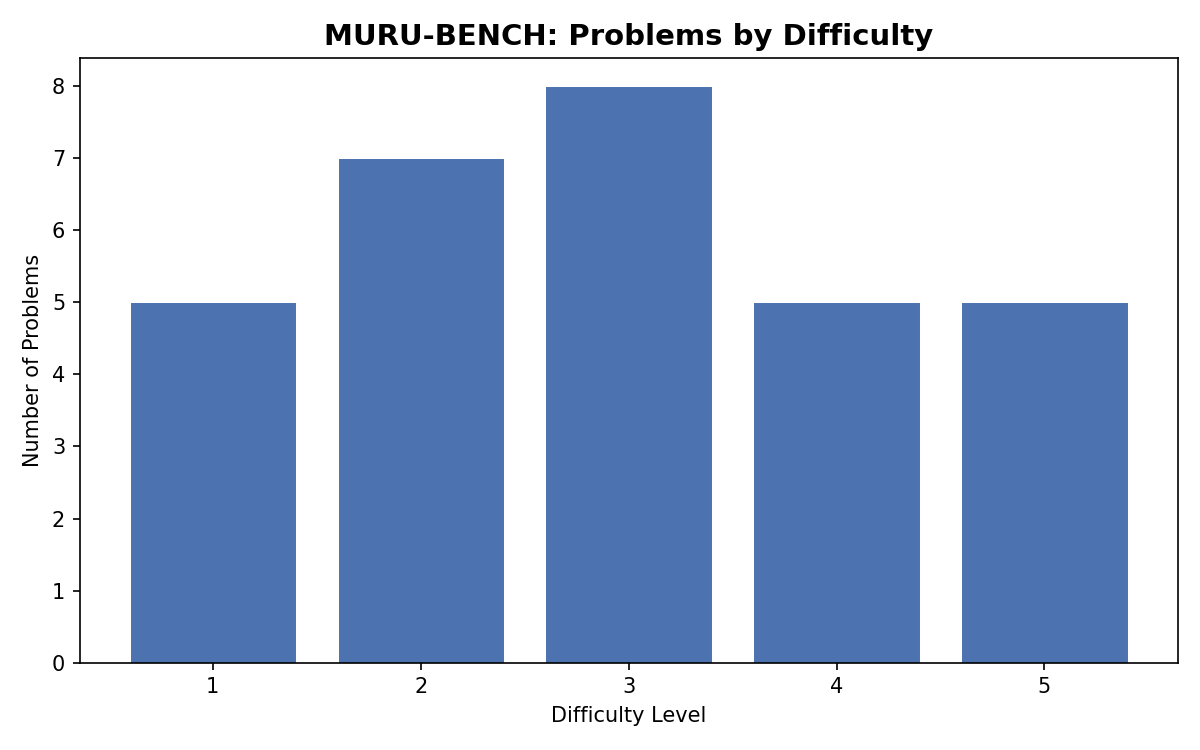
\includegraphics[width=0.6\textwidth]{figures/difficulty_distribution.png}
\caption{Distribution of problems by difficulty level.}
\label{fig:difficulty_dist}
\end{figure}

\begin{figure}[h]
\centering
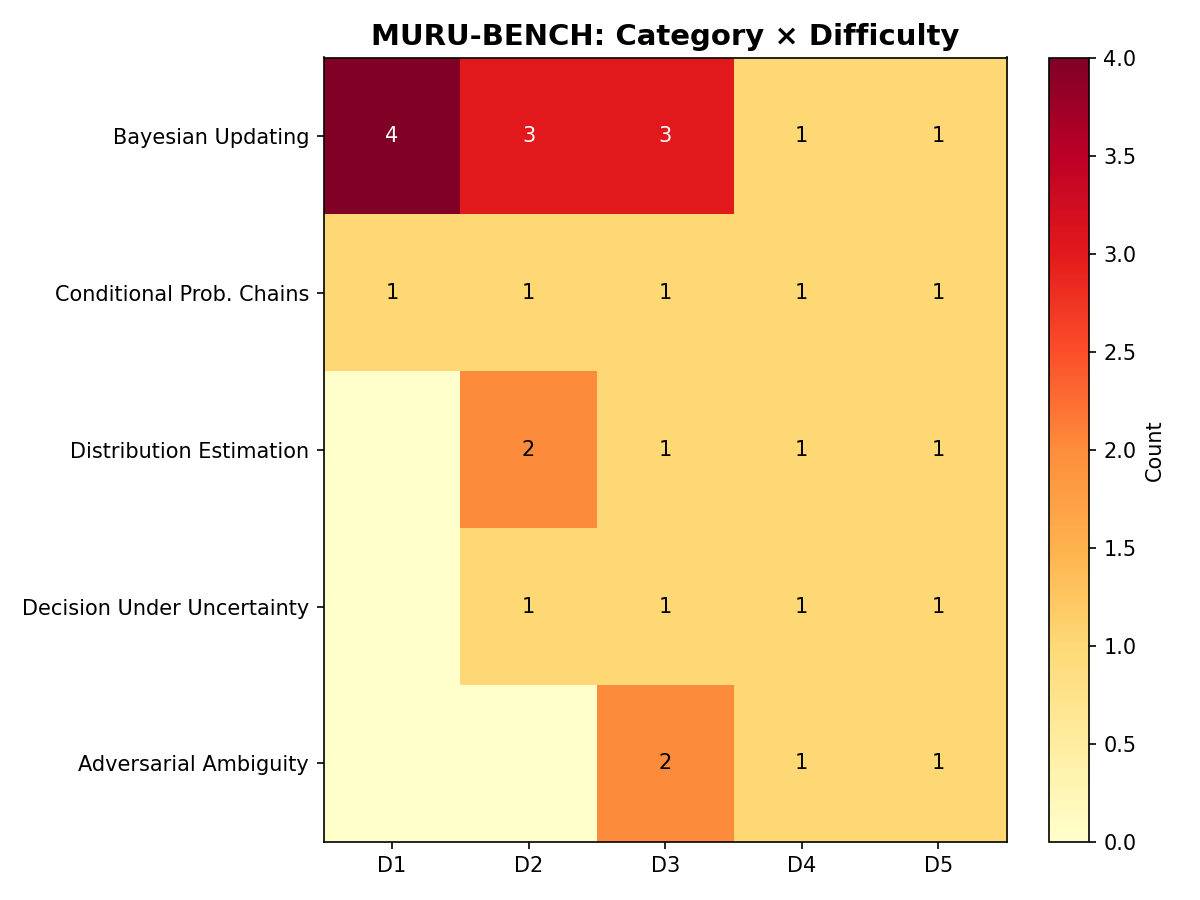
\includegraphics[width=0.7\textwidth]{figures/category_difficulty_heatmap.png}
\caption{Category $\times$ difficulty distribution matrix.}
\label{fig:heatmap}
\end{figure}

\section{Sample Problems}
\label{app:samples}

% TODO: Include 2-3 sample problems from each category


\section{Evaluation Prompts}
\label{app:prompts}

% TODO: Include exact prompts used for each model


\end{document}
